The central finding is the \textbf{data-efficiency crossover}: at
small data, composite is strictly better than AR-only at the AR task;
at large data, AR-only is better. The crossover localises near
$\sim 1{,}000$ problems on this substrate.

\subsection{Setup}

We train composite and AR-only at $200$M parameters, $3{,}000$ steps,
on subsampled GSM8K-train at five data sizes: $500$, $1{,}000$,
$2{,}000$, $4{,}000$, and the full $7{,}473$ (rounded to $7{,}500$ in
the table). At each cell we train $3$--$8$ seeds. We then score
\arNLL{} on a held-out $100$-problem chunk (indices $7{,}000$--$7{,}099$)
and report $\Delta_{\text{NLL}} = \text{NLL}_{\text{composite}} -
\text{NLL}_{\text{AR-only}}$ --- negative numbers favour composite.

\subsection{Results}

\begin{figure}[h]
\centering
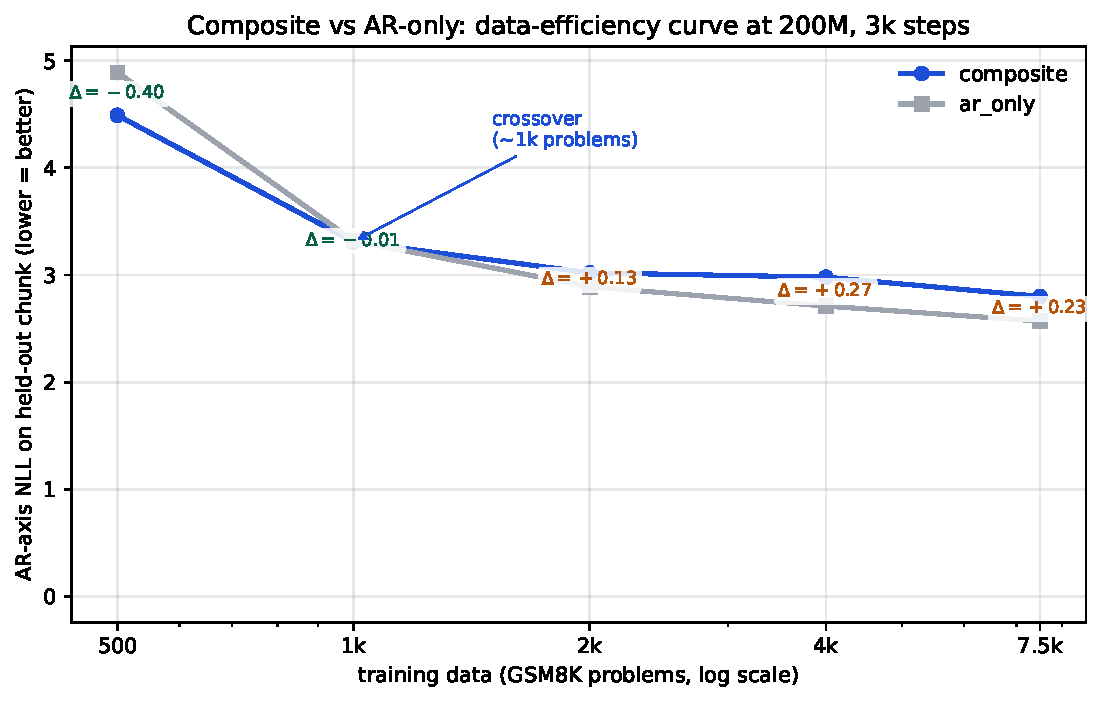
\includegraphics[width=0.82\linewidth]{figures/fig_data_curve.pdf}
\caption{AR-axis NLL at $200$M, $3$k steps, on subsampled GSM8K-train.
Composite (blue) crosses AR-only (gray) near $\sim 1{,}000$ problems.
The $\Delta$ annotations are composite minus AR-only; negative favours
composite. The crossover localisation is the central finding of this
paper.}
\label{fig:data-curve}
\end{figure}

\begin{table}[h]
\centering
\begin{tabular}{lrrrrl}
\toprule
Data size & composite & AR-only & $\Delta_{\text{NLL}}$ & $n$ seeds & seeds agree \\
\midrule
\textbf{500}   & 4.49 & 4.89 & $\mathbf{-0.40}$ & 3 & \textbf{3/3 win} \\
1{,}000        & 3.31 & 3.32 & $-0.01$ & 3 & tied \\
2{,}000        & 3.02 & 2.89 & $+0.13$ & 3 & 3/3 tax \\
4{,}000        & 2.98 & 2.71 & $+0.26$ & 3 & 3/3 tax \\
7{,}500 (full) & 2.80 & 2.57 & $+0.22$ & 8 & consistent tax \\
\bottomrule
\end{tabular}
\caption{AR-axis perplexity vs.\ AR-only baseline at $200$M, $3$k
training steps, on subsampled GSM8K-train. Composite \emph{wins}
decisively in the data-constrained regime ($500$ problems) and loses
mildly above $2{,}000$. The crossover localises to the
$800$--$1{,}200$ band. With $n=3$ seeds we report sign-consistency
(composite is lower/higher for \emph{all} seeds in each non-tied
cell; paired $t(2)$ ranges $|t|=6$--$29$) rather than a
variance-based $\sigma$, which is unstable at this seed count.}
\label{tab:data-curve}
\end{table}

The composite win at $500$ problems ($\Delta = -0.40$ NLL) is the
strongest single positive result in the study. With only $3$ seeds we
do not quote a large-$\sigma$ figure (a variance estimate from $n{=}3$
is itself unstable); instead we report that composite is lower for
\emph{all three} seeds (paired deltas $-0.34, -0.39, -0.46$; paired
$t(2) = -12.1$, $p < 0.01$, treated as a small-$n$ diagnostic rather
than a precise significance). The monotone
trend --- composite advantage declining, then reversing into a small
tax as data grows --- mirrors the DiFFPO~\citep{wei2025diffpo} regime
hypothesis that discrete diffusion's regularising effect is most
beneficial in scarce-data settings.

\paragraph{Crossover localisation.} A separate Phase-E experiment
($3$ seeds each) adds three intermediate data sizes to pin the
crossover to a tighter window. The paired AR-axis delta
(composite $-$ AR-only) climbs monotonically through zero:

\begin{center}
\begin{tabular}{lrrr}
\toprule
problems & $800$ & $1{,}200$ & $1{,}500$ \\
\midrule
$\Delta_\text{NLL}$ (comp $-$ AR) & $\mathbf{-0.165}$ & $+0.052$ & $+0.180$ \\
\bottomrule
\end{tabular}
\end{center}

\noindent Composite still wins the AR axis at $800$ problems
($-0.165$), is within noise at $1{,}200$ ($+0.052$), and pays the tax
by $1{,}500$ ($+0.180$). The sign change localises the crossover to
the $800$--$1{,}200$ problem band, tightening the earlier ``$\sim
1{,}000$'' estimate.

\subsection{Interpretation}

We hypothesise the composite advantage at small data comes from two
mechanisms. First, the diffusion-mode forward pass on masked tokens
exposes the backbone to a denoising objective whose gradient is more
diverse than next-token prediction, acting as a regulariser when the
AR signal is scarce. Second, the bidirectional attention pattern used
in diffusion mode shares the backbone's representational capacity
across multiple objectives, which under-fits less when training data
is limited.

We do \textbf{not} claim this crossover generalises beyond the
GSM8K substrate. Larger-corpus, more-diverse substrates may produce
different curves; further work is needed.
